\documentclass[a4paper,12pt]{article}
\usepackage{latexsym, bbm, float}
\usepackage{amsmath}
\usepackage{amssymb}
\usepackage{amsthm}
\usepackage{graphicx}
\usepackage{fancyhdr}
\usepackage{type1cm}
%\usepackage{times}w
\usepackage{indentfirst}
\usepackage{makeidx}
\usepackage{amsfonts}
%\usepackage{wrapfigure}
\usepackage{hyperref}
\usepackage{color}
\usepackage{natbib}
\usepackage{listings}
\usepackage{xcolor}
\usepackage{tabularx}
\usepackage{graphicx}
\usepackage{subfig}
\usepackage[normalem]{ulem}
\usepackage{times}
\usepackage{ulem}

\setlength{\oddsidemargin}{0.0in}
\setlength{\topmargin}{0.15in}
\setlength{\textwidth}{6.2in}
\setlength{\textheight}{8.75in}

\setlength{\parskip}{0.3cm}


\newcommand{\norm}[1]{\lVert#1\rVert}
\renewcommand{\baselinestretch}{1}
\pagenumbering{arabic}


\newtheorem{thm}{Theorem}[section]
\newtheorem{defn}{Definition}[section]
\newtheorem{lem}{Lemma}[section]
\newtheorem{cor}{Corollary}[section]
\newtheorem{assum}{Assumption}[section]


\theoremstyle{definition}
\newtheorem{exm}{Example}[section]
\newtheorem{remark}{Remark}[section]






%%%%%%%%%% define math symbols %%%%%%%%%%
%% bold and cal letters/LETTERS
\newcommand{\bfm}[1]{\ensuremath{\mathbf{#1}}}
\def\ba{\bfm a}     \def\bA{\bfm A}     \def\cA{{\cal  A}}     \def\calA{{\cal  A}}
\def\bb{\bfm b}     \def\bB{\bfm B}     \def\cB{{\cal  B}}     \def\calB{{\cal  B}}
\def\bc{\bfm c}     \def\bC{\bfm C}     \def\cC{{\cal  C}}     \def\calC{{\cal  C}}
\def\bd{\bfm d}     \def\bD{\bfm D}     \def\cD{{\cal  D}}     \def\calD{{\cal  D}}
\def\be{\bfm e}     \def\bE{\bfm E}     \def\cE{{\cal  E}}     \def\calE{{\cal  E}}
\def\bff{\bfm f}    \def\bF{\bfm F}     \def\cF{{\cal  F}}     \def\calF{{\cal  F}}
\def\bg{\bfm g}     \def\bG{\bfm G}     \def\cG{{\cal  G}}     \def\calG{{\cal  G}}
\def\bh{\bfm h}     \def\bH{\bfm H}     \def\cH{{\cal  H}}     \def\calH{{\cal  H}}
\def\bi{\bfm i}     \def\bI{\bfm I}     \def\cI{{\cal  I}}     \def\calI{{\cal  I}}
\def\bj{\bfm j}     \def\bJ{\bfm J}     \def\cJ{{\cal  J}}     \def\calJ{{\cal  J}}
\def\bk{\bfm k}     \def\bK{\bfm K}     \def\cK{{\cal  K}}     \def\calK{{\cal  K}}
\def\bl{\bfm l}     \def\bL{\bfm L}     \def\cL{{\cal  L}}     \def\calL{{\cal  L}}
\def\bm{\bfm m}     \def\bM{\bfm M}     \def\cM{{\cal  M}}     \def\calM{{\cal  M}}
\def\bn{\bfm n}     \def\bN{\bfm N}     \def\cN{{\cal  N}}     \def\calN{{\cal  N}}
\def\bo{\bfm o}     \def\bO{\bfm O}     \def\cO{{\cal  O}}     \def\calO{{\cal  O}}
\def\bp{\bfm p}     \def\bP{\bfm P}     \def\cP{{\cal  P}}     \def\calP{{\cal  P}}
\def\bq{\bfm q}     \def\bQ{\bfm Q}     \def\cQ{{\cal  Q}}     \def\calQ{{\cal  Q}}
\def\br{\bfm r}     \def\bR{\bfm R}     \def\cR{{\cal  R}}     \def\calR{{\cal  R}}
\def\bs{\bfm s}     \def\bS{\bfm S}     \def\cS{{\cal  S}}     \def\calS{{\cal  S}}
\def\bt{\bfm t}     \def\bT{\bfm T}     \def\cT{{\cal  T}}     \def\calT{{\cal  T}}
\def\bu{\bfm u}     \def\bU{\bfm U}     \def\cU{{\cal  U}}     \def\calU{{\cal  U}}
\def\bv{\bfm v}     \def\bV{\bfm V}     \def\cV{{\cal  V}}     \def\calV{{\cal  V}}
\def\bw{\bfm w}     \def\bW{\bfm W}     \def\cW{{\cal  W}}     \def\calW{{\cal  W}}
\def\bx{\bfm x}     \def\bX{\bfm X}     \def\cX{{\cal  X}}     \def\calX{{\cal  X}}
\def\by{\bfm y}     \def\bY{\bfm Y}     \def\cY{{\cal  Y}}     \def\calY{{\cal  Y}}
\def\bz{\bfm z}     \def\bZ{\bfm Z}     \def\cZ{{\cal  Z}}     \def\calZ{{\cal  Z}}
\def\bzero{\bfm 0}

% \boldsymbol{greek letters}
\newcommand{\bfsym}[1]{\ensuremath{\boldsymbol{#1}}}
\def \balpha   {\bfsym{\alpha}}       \def \bbeta    {\bfsym{\beta}}
\def \bgamma   {\bfsym{\gamma}}       \def \bdelta   {\bfsym{\delta}}
\def \bepsilon {\bfsym{\epsilon}}     \def \bzeta    {\bfsym{\zeta}}
\def \betta    {\bfsym{\eta}}         \def \btheta   {\bfsym{\theta}}
\def \biota    {\bfsym{\iota}}        \def \bkappa   {\bfsym{\kappa}}
\def \blambda  {\bfsym{\lambda}}      \def \bmu      {\bfsym{\mu}}
\def \bnu      {\bfsym{\nu}}          \def \bxi      {\bfsym{\xi}}
\def \bomicron {\bfsym{\omicron}}     \def \bpi      {\bfsym{\pi}}
\def \brho     {\bfsym{\rho}}         \def \bsigma   {\bfsym{\sigma}}
\def \btau     {\bfsym{\tau}}         \def \bupsilon {\bfsym{\upsilon}}
\def \bphi     {\bfsym{\phi}}         \def \bchi     {\bfsym{\chi}}
\def \bpsi     {\bfsym{\psi}}         \def \bomega   {\bfsym{\omega}}
\def \beps     {\bfsym \varepsilon}

% \boldsymbol{GREEK LETTERS}
\def \bGamma   {\bfsym{\Gamma}}       \def \bDelta   {\bfsym{\Delta}}
\def \bTheta   {\bfsym{\Theta}}       \def \bLambda  {\bfsym{\Lambda}}
\def \bXi      {\bfsym{\Xi}}          \def \bPi      {\bfsym{\Pi}}
\def \bSigma   {\bfsym{\Sigma}}       \def \bUpsilon {\bfsym{\Upsilon}}
\def \bPhi     {\bfsym{\Phi}}         \def \bPsi     {\bfsym{\Psi}}
\def \bOmega   {\bfsym{\Omega}}

% \hat{greek letters}
\renewcommand{\hat}{\widehat}
\def \halpha   {\hat{\alpha}}         \def \hbeta    {\hat{\beta}}
\def \hgamma   {\hat{\gamma}}         \def \hdelta   {\hat{\delta}}
\def \hepsilon {\hat{\epsilon}}       \def \hzeta    {\hat{\zeta}}
\def \heta     {\hat{\eta}}           \def \htheta   {\hat{\theta}}
\def \hiota    {\hat{\iota}}          \def \hkappa   {\hat{\kappa}}
\def \hlambda  {\hat{\lambda}}        \def \hmu      {\hat{\mu}}
\def \hnu      {\hat{\nu}}            \def \hxi      {\hat{\xi}}
\def \homicron {\hat{\omicron}}       \def \hpi      {\hat{\pi}}
\def \hrho     {\hat{\rho}}           \def \hsigma   {\hat{\sigma}}
\def \htau     {\hat{\tau}}           \def \hupsilon {\hat{\upsilon}}
\def \hphi     {\hat{\phi}}           \def \hchi     {\hat{\chi}}
\def \hpsi     {\hat{\psi}}           \def \homega   {\hat{\omega}}
\def \heps     {\hat{\heps}}

% \hat{\boldsymbol{greek letters}}
\def \hbalpha   {\hat{\balpha}}       \def \hbbeta    {\hat{\bbeta}}
\def \hbgamma   {\hat{\bgamma}}       \def \hbdelta   {\hat{\bdelta}}
\def \hbepsilon {\hat{\bepsilon}}     \def \hbzeta    {\hat{\bzeta}}
\def \hbeta     {\hat{\betta}}        \def \hbtheta   {\hat{\btheta}}
\def \hbiota    {\hat{\biota}}        \def \hbkappa   {\hat{\bkappa}}
\def \hblambda  {\hat{\blambda}}      \def \hbmu      {\hat{\bmu}}
\def \hbnu      {\hat{\bnu}}          \def \hbxi      {\hat{\bxi}}
\def \hbomicron {\hat{\bomicron}}     \def \hbpi      {\hat{\bpi}}
\def \hbrho     {\hat{\brho}}         \def \hbsigma   {\hat{\bsigma}}
\def \hbtau     {\hat{\btau}}         \def \hbupsilon {\hat{\bupsilon}}
\def \hbphi     {\hat{\bphi}}         \def \hbchi     {\hat{\bchi}}
\def \hbpsi     {\hat{\bpsi}}         \def \hbomega   {\hat{\bomega}}
\def \hbeps     {\hat{\beps}}

% \hat{\boldsymbol{GREEK LETTERS}}
\def \hbGamma   {\hat{\bGamma}}       \def \hbDelta   {\hat{\bDelta}}
\def \hbTheta   {\hat{\bTheta}}       \def \hbLambda  {\hat{\bLambda}}
\def \hbXi      {\hat{\bXi}}          \def \hbPi      {\hat{\bPi}}
\def \hbSigma   {\hat{\bSigma}}       \def \hbUpsilon {\hat{\bUpsilon}}
\def \hbPhi     {\hat{\bPhi}}         \def \hbPsi     {\hat{\bPsi}}
\def \hbOmega   {\hat{\bOmega}}


\newcommand{\lzeronorm}[1]{\lVert#1\rVert_0}
\newcommand{\lonenorm}[1]{\lVert#1\rVert_1}
\newcommand{\ltwonorm}[1]{\lVert#1\rVert_2}
\newcommand{\lfournorm}[1]{\lVert#1\rVert_4}
\newcommand{\opnorm}[1]{\lVert#1\rVert_{op}}
\newcommand{\fnorm}[1]{\lVert#1\rVert_F}
\newcommand{\nnorm}[1]{\lVert#1\rVert_N}
\newcommand{\supnorm}[1]{ \lVert#1  \rVert_{\max}}
\newcommand{\inn}[1]{\langle #1 \rangle}
\newcommand{\truncate}[1]{\sgn(#1)(|#1|\wedge \tau)}
\newcommand{\shrunk}[1]{#1 (\|#1\|_2 \wedge \tau)/\ltwonorm{#1}}
\newcommand{\shrunkt}[1]{#1^T \; (\|#1\|_2 \wedge \tau)/\ltwonorm{#1}}
\newcommand{\beq}  {\begin{equation}}
\newcommand{\eeq}  {\end{equation}}

\DeclareMathOperator*{\argmax}{argmax}
\DeclareMathOperator*{\argmin}{argmin}
\DeclareMathOperator{\corr}{corr}
\DeclareMathOperator{\cov}{cov}
\DeclareMathOperator{\Cov}{Cov}
\DeclareMathOperator{\Dev}{Dev}
\DeclareMathOperator{\diag}{diag}
\DeclareMathOperator{\E}{E}
\DeclareMathOperator{\logit}{logit}
\DeclareMathOperator{\rank}{rank}
\DeclareMathOperator{\RSS}{RSS}
\DeclareMathOperator{\sgn}{sgn}
\DeclareMathOperator{\supp}{supp}
\DeclareMathOperator{\Var}{Var}
\DeclareMathOperator{\var}{var}
\DeclareMathOperator{\SE}{SE}
\DeclareMathOperator{\tr}{tr}

\def \var   {\mbox{var}}
\def \corr  {\mbox{corr}}
\def \rase  {\mbox{RASE}}
\def \Cov   {\mbox{Cov}}
\def \C     {\mbox{const.}\quad}
\def \MSE   {\mbox{MSE}}
\def \MISE  {\mbox{MISE}}
\def \AMISE {\mbox{AMISE}}
\def \SE    {\mbox{SE}}
\def \se    {\mbox{SE}}
\def \andd  {\mbox{and}}
\def \logit {\mbox{logit}}
\def \new   {\mbox{new}}
\def \say   {\mbox{(say)}}
\def \MLE   {\mbox{\smallfont{MLE}}}
\def \U     {\mbox{\smallfont{U}}}
\def \sgn   {\mbox{sgn}}
\def \rcv   {{\rm RCV}}
\def \lasso {{\rm LASSO}}
\def \scad  {{\rm SCAD}}

\def \betaa    {\bbeta_{\alpha}^{\ast}}
\def \betas    {\bbeta^{\ast}}
\def \betah    {\bbeta_{\alpha}^{h}}
\def \betac    {\bbeta_{\alpha}^{c}}
\def \betacs   {\bbeta_{\alpha}^{c\ast}}
\def \sqLogpN  {\sqrt{(\log p)/n}}
\def \la       {\ell_{\alpha}}
\def \kl       {\kappa_{\cL}}
\def \ku       {\kappa_u}
\def \ko       {\kappa_0}
\def \Rd       {\mathbb{R}^d}
\def \Rdd	{\mathbb{R}^{d_1\times d_2}}
\def \RR	{\mathbb{R}}
\def \NN {\mathbb{N}}
\def \fd       {f_{\bDelta}}
\def \gd       {g_{\bDelta}}
\def \Rq       {R_{q}}
\def \bbP      {\mathbb{P}}
\def \bbS      {\mathbb{S}}
\def \sidx     {\sup_{(\bbeta,\bDelta)\in A'\cap \bDelta \in \bbS_1(\tau)}}
\def \vec	{\text{vec}}
\def \mat {\text{mat}}
\def \hcov	{\hat\Sigma^h_{yx_j}(\alpha)}
\def \ind {1}
\def \Tr {\text{Tr}}
\def \bbX {\mathbb{X}}
\def \bbY {\mathbb{Y}}
% Custom new command
\newcommand\redsout{\bgroup\markoverwith{\textcolor{red}{\rule[0.5ex]{2pt}{1pt}}}\ULon}

\title{COMS W 4111 Project 1 Proposal}
\author{Xiaoyang Song  \&  Han Liu}
\date{FA 2022}

\begin{document}
\maketitle
\section{Domain \& Short Introduction}
Our project focuses on the domain of restaurant inspections and ratings at New York City, and the source dataset is obtained from the website \href{https://data.cityofnewyork.us/Health/DOHMH-New-York-City-Restaurant-Inspection-Results/43nn-pn8j}{NYC Open Data}. In our project, we aim to first create a database where all relevant data about NYC restaurant inspections and ratings will be stored for users to browse; then we desire to model user information and their reviews to the restaurants, which will be added interactively and dynamically to our database by users. With that being said, our web application will also have login function. In general, by completing these goals, we intend to provide our users an opportunity to interactively review the restaurant recent government inspection results, violation records, and ratings and add their favorite/disliked restaurants to their preference/hate list. For example, if users want to know something about "Chipotle", then all the reviews, inspection records, ratings, and violations associated with "Chipotle" can be retrieved for users to read; furthermore, they can add "Chipotle" to their list of favorite restaurant or write a review for "Chipotle" if they want to. In addition, our web application is useful for different groups of people. For instance, government staffs and inspectors may use this application to check which restaurants have violated certain regulations before when determining their inspection plan and target; for researchers and data scientists, they may use this application to investigate which type of inspection can find violations the most and make some statistical inference based on that. As for our database design, we currently have 7 entity sets and 8 relationship sets with bunch of constraints. For example, \textit{Restaurant}, \textit{Reviews}, and \textit{Users} are three of the entity sets we relied on. Below are some relationship examples that our model can effectively capture:
\vspace{-0.4cm}
\begin{itemize}
    \item A \textit{User} can \textbf{Like} any number of \textit{Restaurant}.
    \vspace{-0.2cm}
    \item A \textit{User} can \textbf{Post} any number of \textit{Reviews} to a certain \textit{Restaurant}. 
    \vspace{-0.2cm}
    \item A \textit{Review} can not exist without a \textit{User}.
\end{itemize}
\vspace{-0.4cm}
Other entity sets we made are \textit{Locations}, \textit{Inspection}, \textit{Grades}, and \textit{Violations}. With these entity sets and relationship sets, we can accomplish our goals perfectly. The detailed explanation of ER modeling can be found on the next page, and the revision made after TA meetings can be found in Appendix A.

\newpage
\section{ER Diagram Design}
\subsection{Introduction to Entity Sets}
In our design of the database, we include $7$ entity sets in total: \textbf{Users}, \textbf{Restaurant}, \textbf{Locations}, \textbf{Review}, \textbf{Inspection}, \textbf{Grade}, and \textbf{Violation}. A detailed description and design logic are introduced below:
\begin{enumerate}
    \item \textbf{User:} \textbf{User} keeps track of the information of users to our web-app. 
    \begin{itemize}
        \item \textit{user\_id} (int): globally unique primary key.
        \item \textit{account\_name} (text) [not null]: users' account name.
        \item \textit{passcode} (text) [not null]: users' passcode.
        \item \textit{dob} (DATE): date of birth.
        \item \textit{district} (text): the district that the user belongs in NYC. Note that the value of this attribute can only be one of the NYC district set\footnotemark[1]\footnotetext[1]{NYC district sets = \{'Manhattan', 'Bronx', 'Brooklyn', 'Queens', 'Staten Island'\}}. We keep track of this so that we can send recommendation to the users based on their geographic location.
    \end{itemize}
    \item \textbf{Restaurant:} \textbf{Restaurant} keeps track of the information of restaurant.
    \begin{itemize}
        \item \textit{r\_id} (int): globally unique primary key.
        \item \textit{DBA} (text) [not null]: the acronym (i.e. name) of the restaurant.
        \item \textit{phone\_number} (VARCHAR(10)): the phone number of restaurant. Note that we only focus on NYC restaurant so a 10-digit phone number is enough.
        \item \textit{cuisine} (text): description of the cuisine.
    \end{itemize}
    \item \textbf{Location:} 
    \begin{itemize}
        \item \textit{l\_id} (int): globally unique primary key.
        \item \textit{district} (text): the value of this field must belong to the NYC district sets \footnotemark[1].
        \item \textit{zipcode} (VARCHAR(5)): zipcode of the location.
        \item \textit{street} (text): street of the location.
        \item \textit{building} (text): building of the location.
    \end{itemize}

    \item \textbf{Reviews:} \textbf{Reviews} contain users' review to restaurants.
    \begin{itemize}
        \item \textit{rev\_id} (int): globally unique primary key.
        \item \textit{content} (text) [not null]: description of the reviews. 
        % \item \textit{rev\_time} (DATE): time that this review is made.
        % \item \textit{street} (text): street of the location.
        % \item \textit{building} (text): building of the location.
    \end{itemize}
    
    \item \textbf{Inspection:} \textbf{Inspection} keeps track of the inspection records of restaurants.
     \begin{itemize}
        \item \textit{i\_id} (int): globally unique primary key.
        \item \textit{i\_type} (text): type of the inspection.
    \end{itemize}
    \item \textbf{Grade:} \textbf{Grade} keeps track of the grades of restaurants.
    \begin{itemize}
        \item \textit{g\_id} (int): globally unique primary key.
        \item \textit{grade} (CHAR(1)) [not null]: grade level. Note that the value of this attribute must belong to one of the grade set \footnotemark[1]\footnotetext[1]{grade set = \{'A', 'B', 'C', 'P', 'Z'\}}.
        \item \textit{score} (float): specific score.
    \end{itemize}
    \item \textbf{Violation:}
    \begin{itemize}
        \item \textit{v\_id} (int): globally unique primary key.
        \item \textit{code} (text): government code that specifies the violation.
        \item \textit{v\_description} (text): description of the violation.
        \item \textit{critical\_flag} (text): note that this attribute must belong to the flag set \footnotemark[2]\footnotetext[2]{flag set = \{'Critical', 'Not Critical', 'Not Applicable'\}}.
    \end{itemize} 
\end{enumerate}

\subsection{Introduction to Relationship Sets}
In total, we have $8$ Relationship sets and many constraints imposed on them.
\begin{enumerate}
    \item \textit{Restaurant} \textbf{Locate} at \textit{Location}: A restaurant can locate at exactly one location, while one location may hold multiple restaurant. One example for this is food court where multiple restaurant has the same location. Note that we treat franchise stores at different locations as different \textit{Restaurant} entities.
    \item \textit{User} \textbf{Post} \textit{Reviews}: A user can post many reviews; however, a review can be posted by only one user. Furthermore, when a user is deleted, the review should also goes away so we make review a weak entity of user. Furthermore, we can keep track of when the review is posted.
    \item \textit{Restaurant} \textbf{Own} \textit{Reviews}: A restaurant can have many reviews; however, a review must be made to exactly one restaurant (We make this assumption to avoid reviews which contain multiple restaurants, which is not very informative in reality). In addition, when a restaurant is deleted, its reviews should also go away, so we make review a weak entity of restaurant as well \footnotemark[3]\footnotetext[3]{Note that \textit{Review} is actually a weak entity of two entity sets, so it will be deleted on cascade if either \textit{User} or \textit{Restaurant} is deleted}. 
    \item \textit{User} \textbf{Like} \textit{Restaurant}: A user can like many restaurants, and a restaurant can be liked by many users. By keep tracking this relationship, we keep track of the restaurant that a user like; we can provide users list of restaurant they like in our web application easily by querying on this relationship sets in our database.
    \item \textit{User} \textbf{Dislike} \textit{Restaurant}: A user can dislike many restaurants, and a restaurant can be disliked by many users. The intuition behind this relationship set is very similar to that of the \textbf{Like} relationship set.
    \item \textit{Restaurant} \textbf{graded} by \textit{Grade}: A restaurant can have many grades, and a grade can be associated with many restaurants. We also track when this grading action happens.
    \item \textit{Restaurant} \textbf{inspected} by \textit{Inspection}: A restaurant can have many inspections at any time described by inspection time, and an inspection can be done on multiple restaurants. 
    \item \textit{Violation} is \textbf{Found} by \textit{Inspection}: A violation can be found by multiple inspection, and an inspection can find any number of violations. 
    \item \textit{Restaurant} \textbf{violate} \textit{Violation}: A restaurant can have any number of violations, and a violation can be found in any number of restaurants.
\end{enumerate}
Note that the last three relationship sets together enable the users to interactive query on any of them for useful information. For instance, for a given restaurant, a user can check whether it has any violation records and also its recent inspection records. In addition, users like the government staffs can also easily check which restaurants violate certain rules given an instance of violation. The combination of these three entity sets are very powerful in reality and can be used for different people including government staffs and normal citizens.

\subsection{ER-Diagram}
The ER-Diagram is provided on the next page. As mentioned in lecture, the ER-Diagram just aims to show the basic structure of the database so complicated check constraints are not shown on that. But to make things clearer, basic data types are drawn out.


\begin{figure}
    \centering
    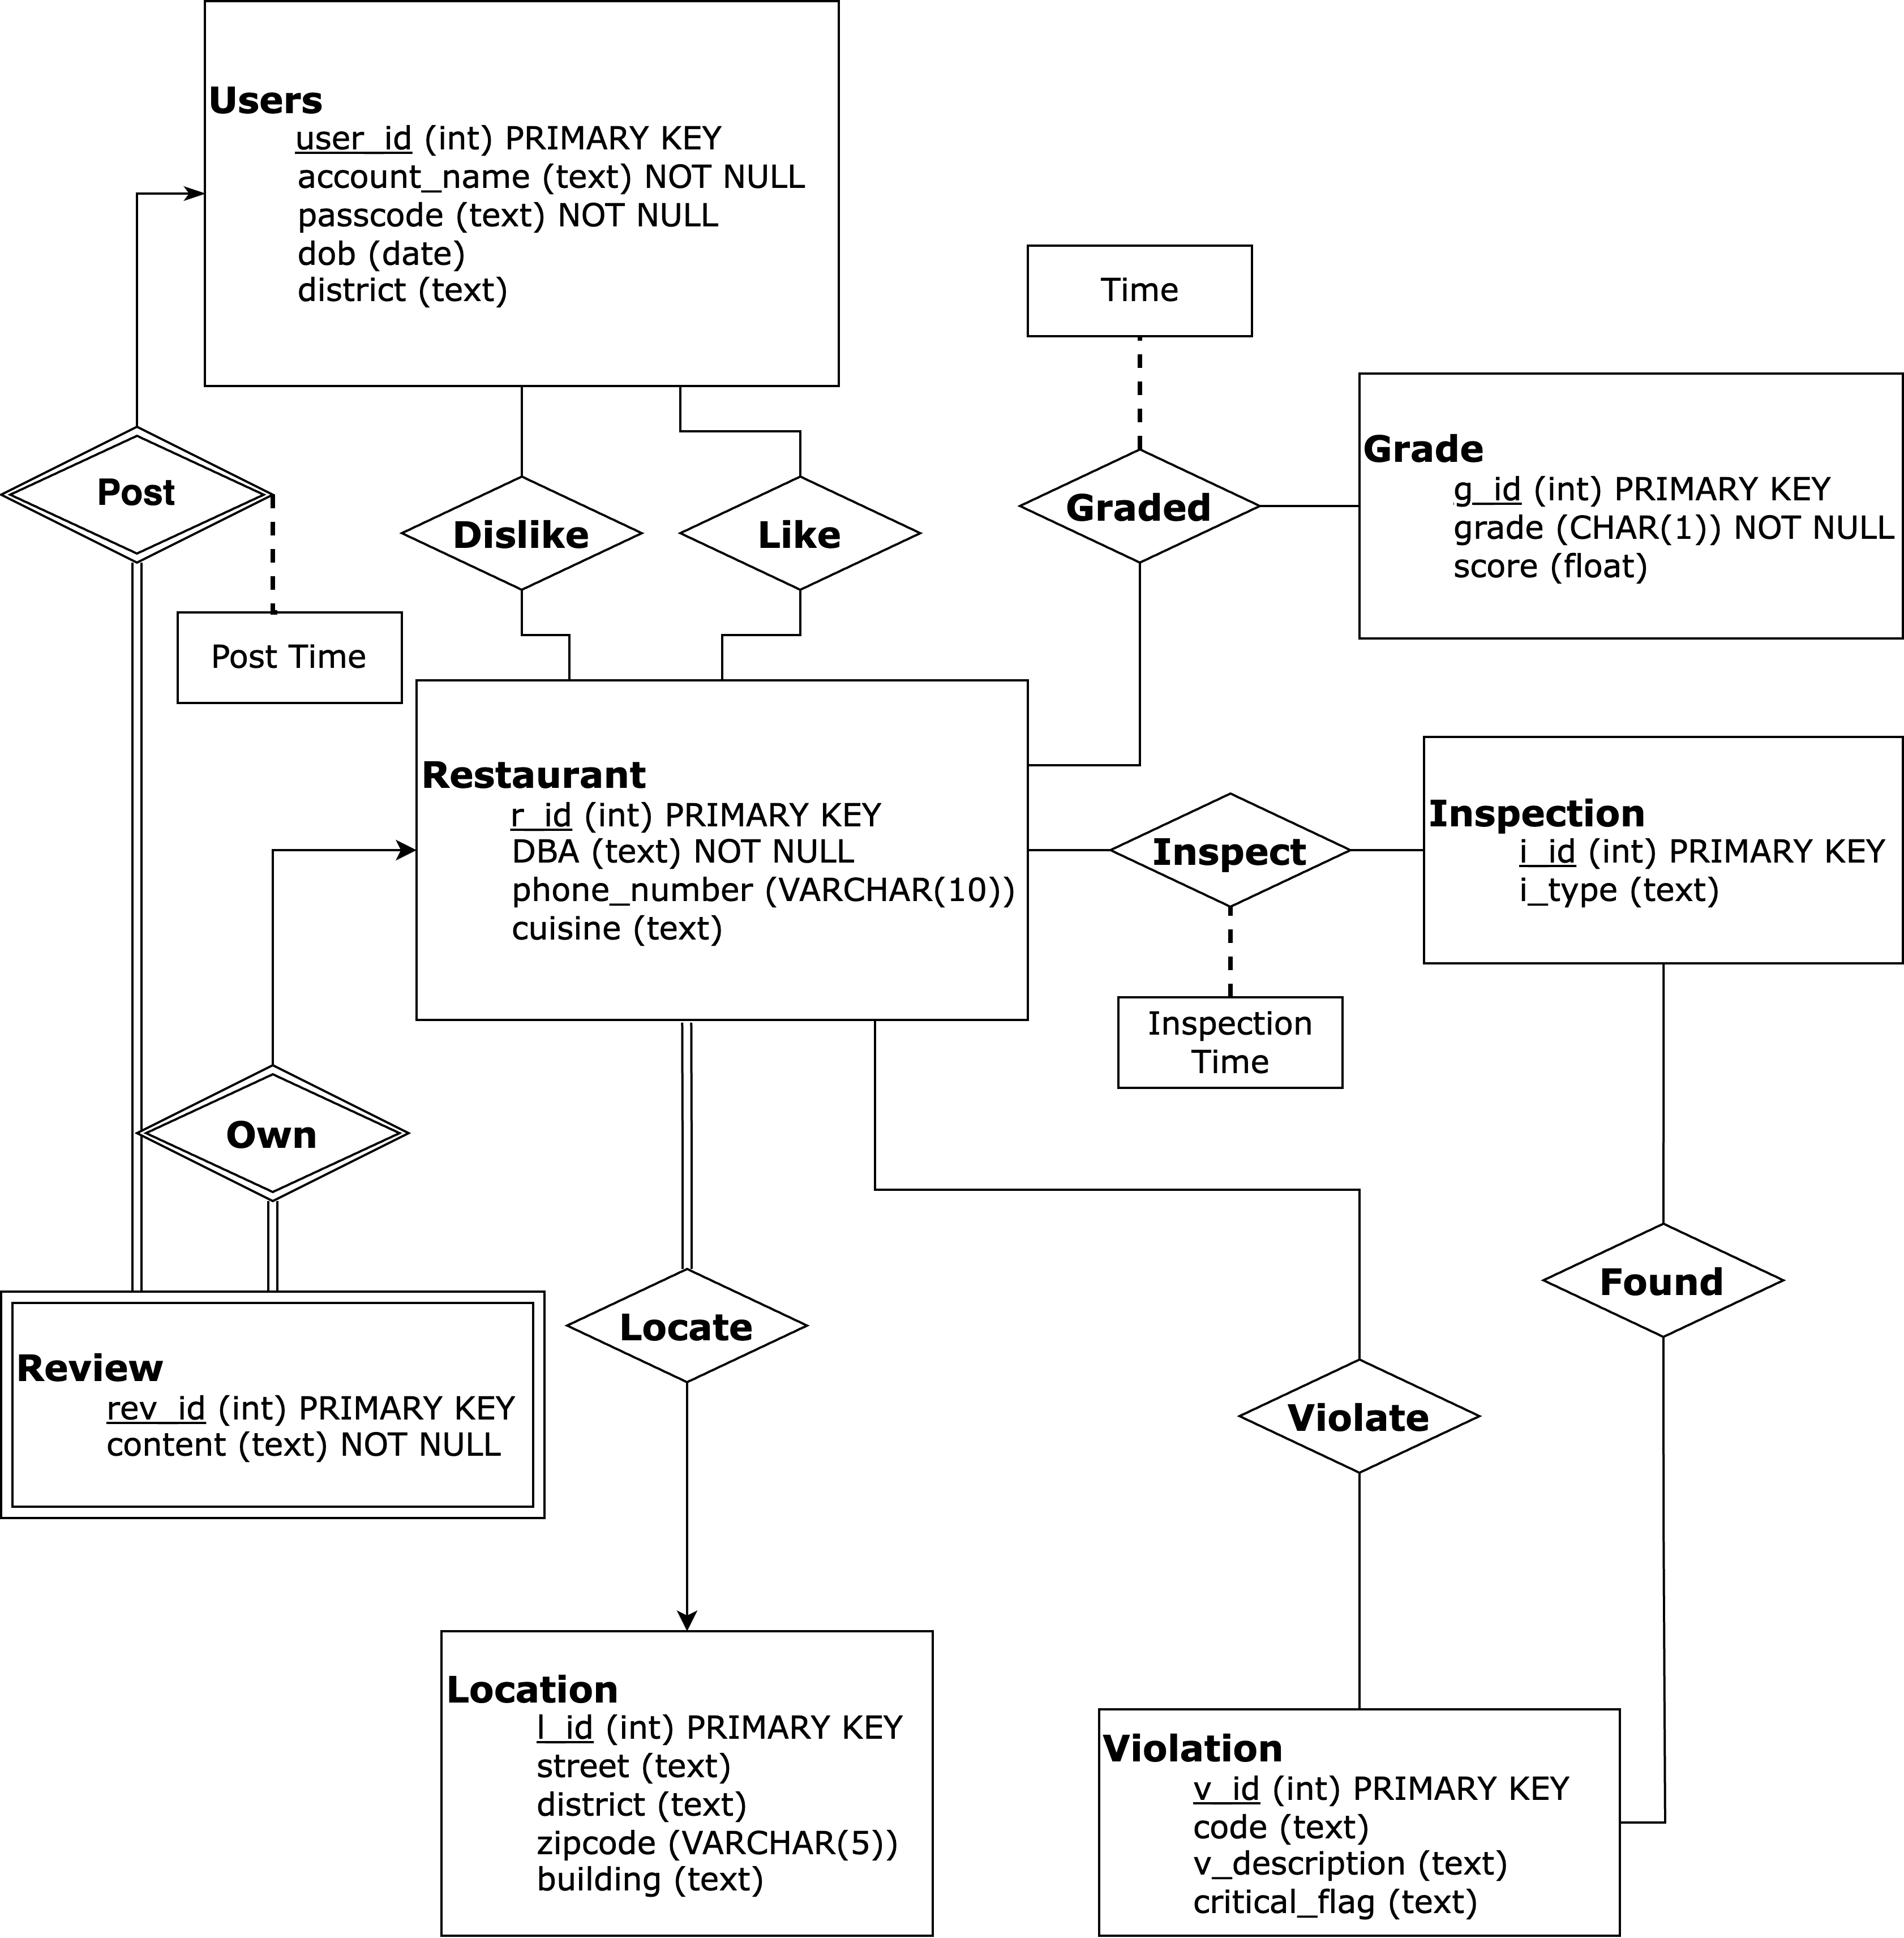
\includegraphics[scale = 0.75]{Project1_ER.png}
    \caption{ER Diagram}
    \label{fig:er}
\end{figure}

\newpage
\section{Relational Schema Translation}
There are several caveats about our translation:
\vspace{-0.4cm}
\begin{enumerate}
    \item When translating the \textbf{Like} and \textbf{Dislike}, we combine them into one to make things more efficient, but the functionalities are unchanged.
    \item A very small portion of the variable names are not fully-consistent with Diagram because some variable names like "Locate" are treated as keyword in SQL compiler that I used. However, the difference is very minor and our code makes it clear, so you should be able to find its correspondence in ER-Diagram easily.
\end{enumerate}
The below are the code snippets (please check Figure 2 to Figure 6) for translating ER-Diagram to relational model. You can also visit our \href{https://github.com/Xiaoyang-Song/NYC-Restaurant-Inspection-Database/blob/main/p1.SQL}{Github Repository} to view this code. (https://github.com/Xiaoyang-Song/NYC-Restaurant-Inspection-Database/blob/main/p1.SQL)

\begin{figure}[h]
    \centering
    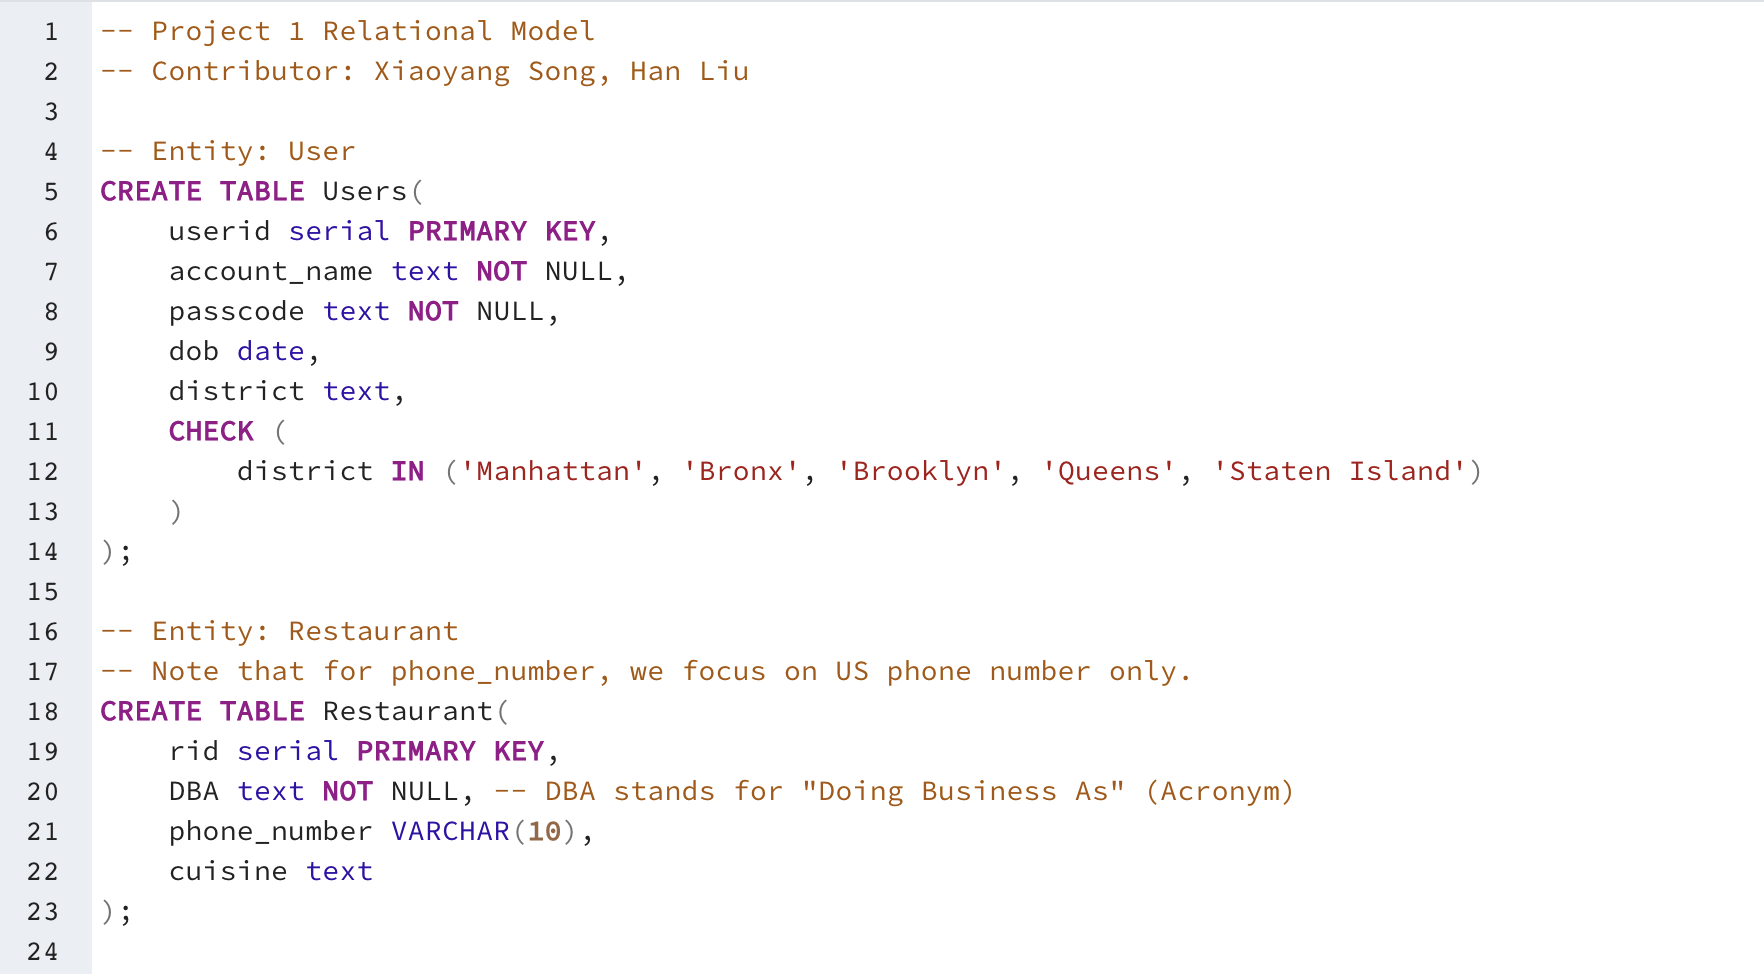
\includegraphics[scale = 0.58]{1.png}
    \caption{Relational Model}
    \label{fig:1}
\end{figure}
\begin{figure}[h]
    \centering
    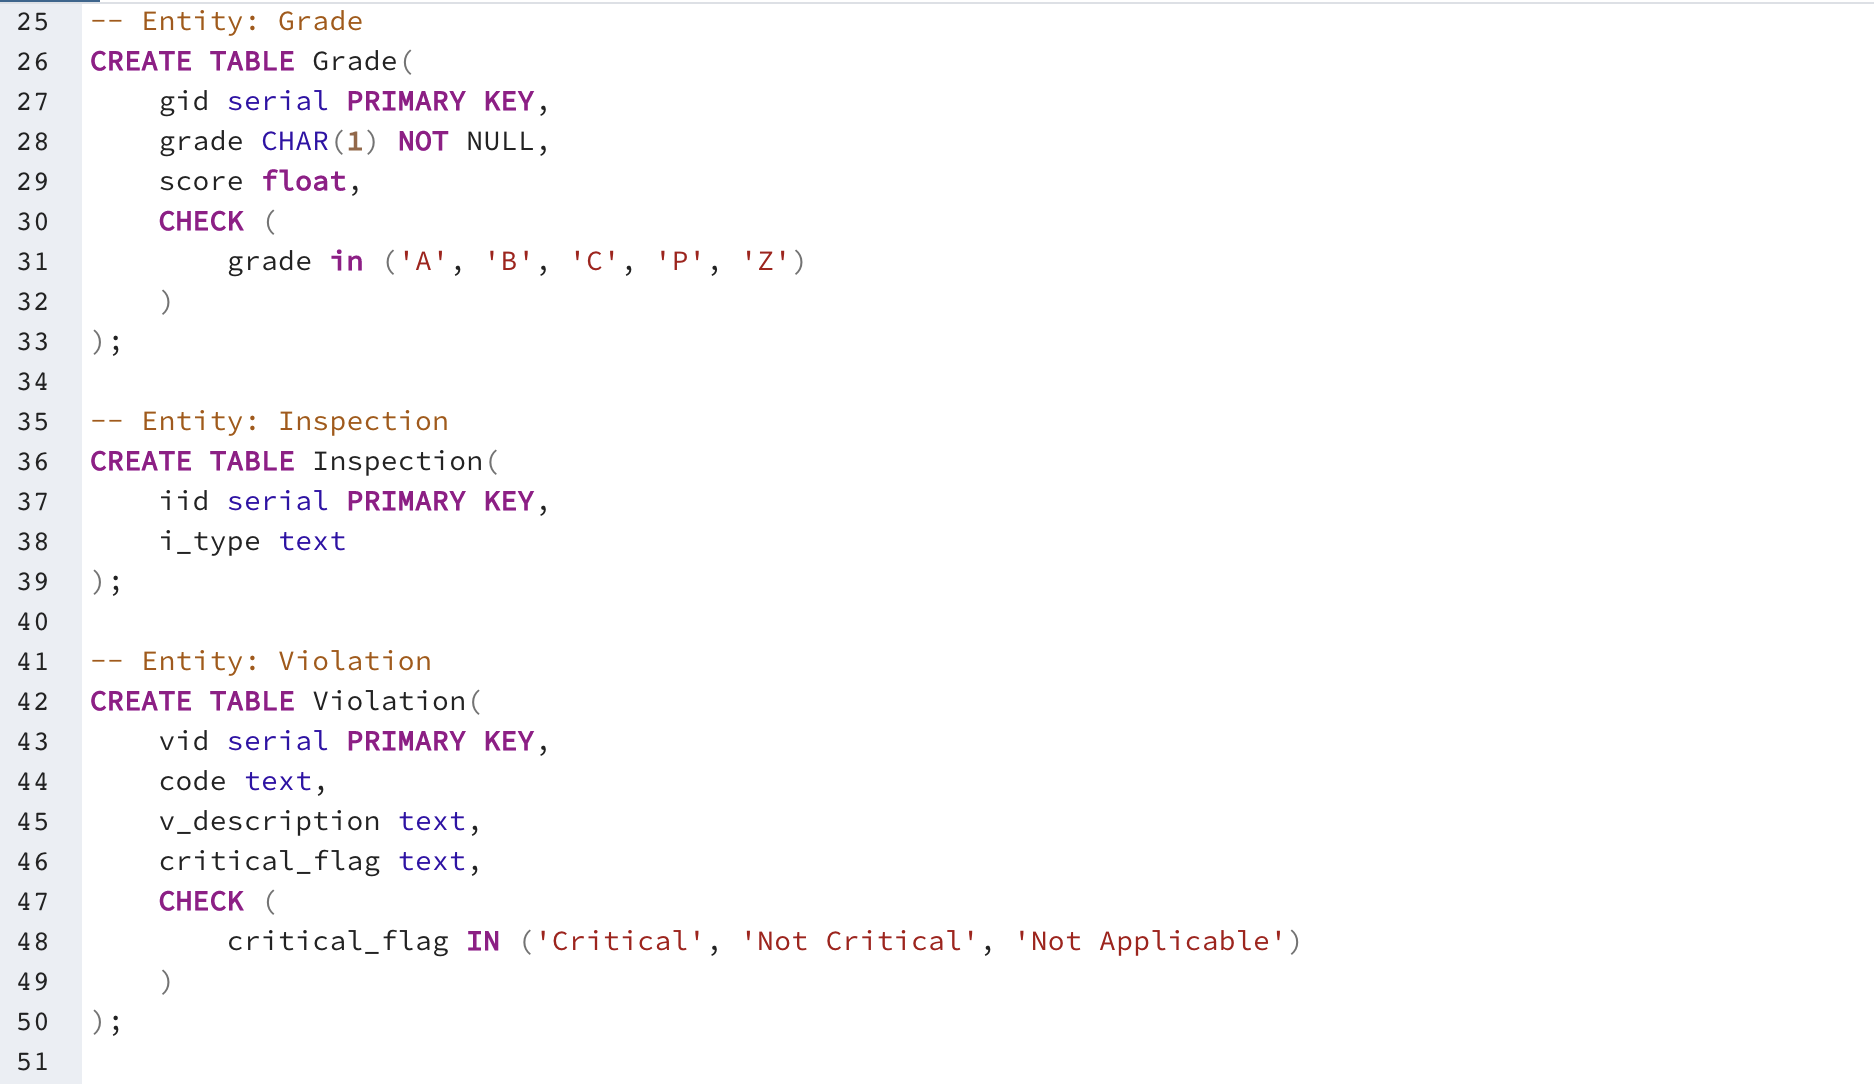
\includegraphics[scale = 0.58]{2.png}
    \caption{Relational Model}
    \label{fig:2}
\end{figure}
\begin{figure}[h]
    \centering
    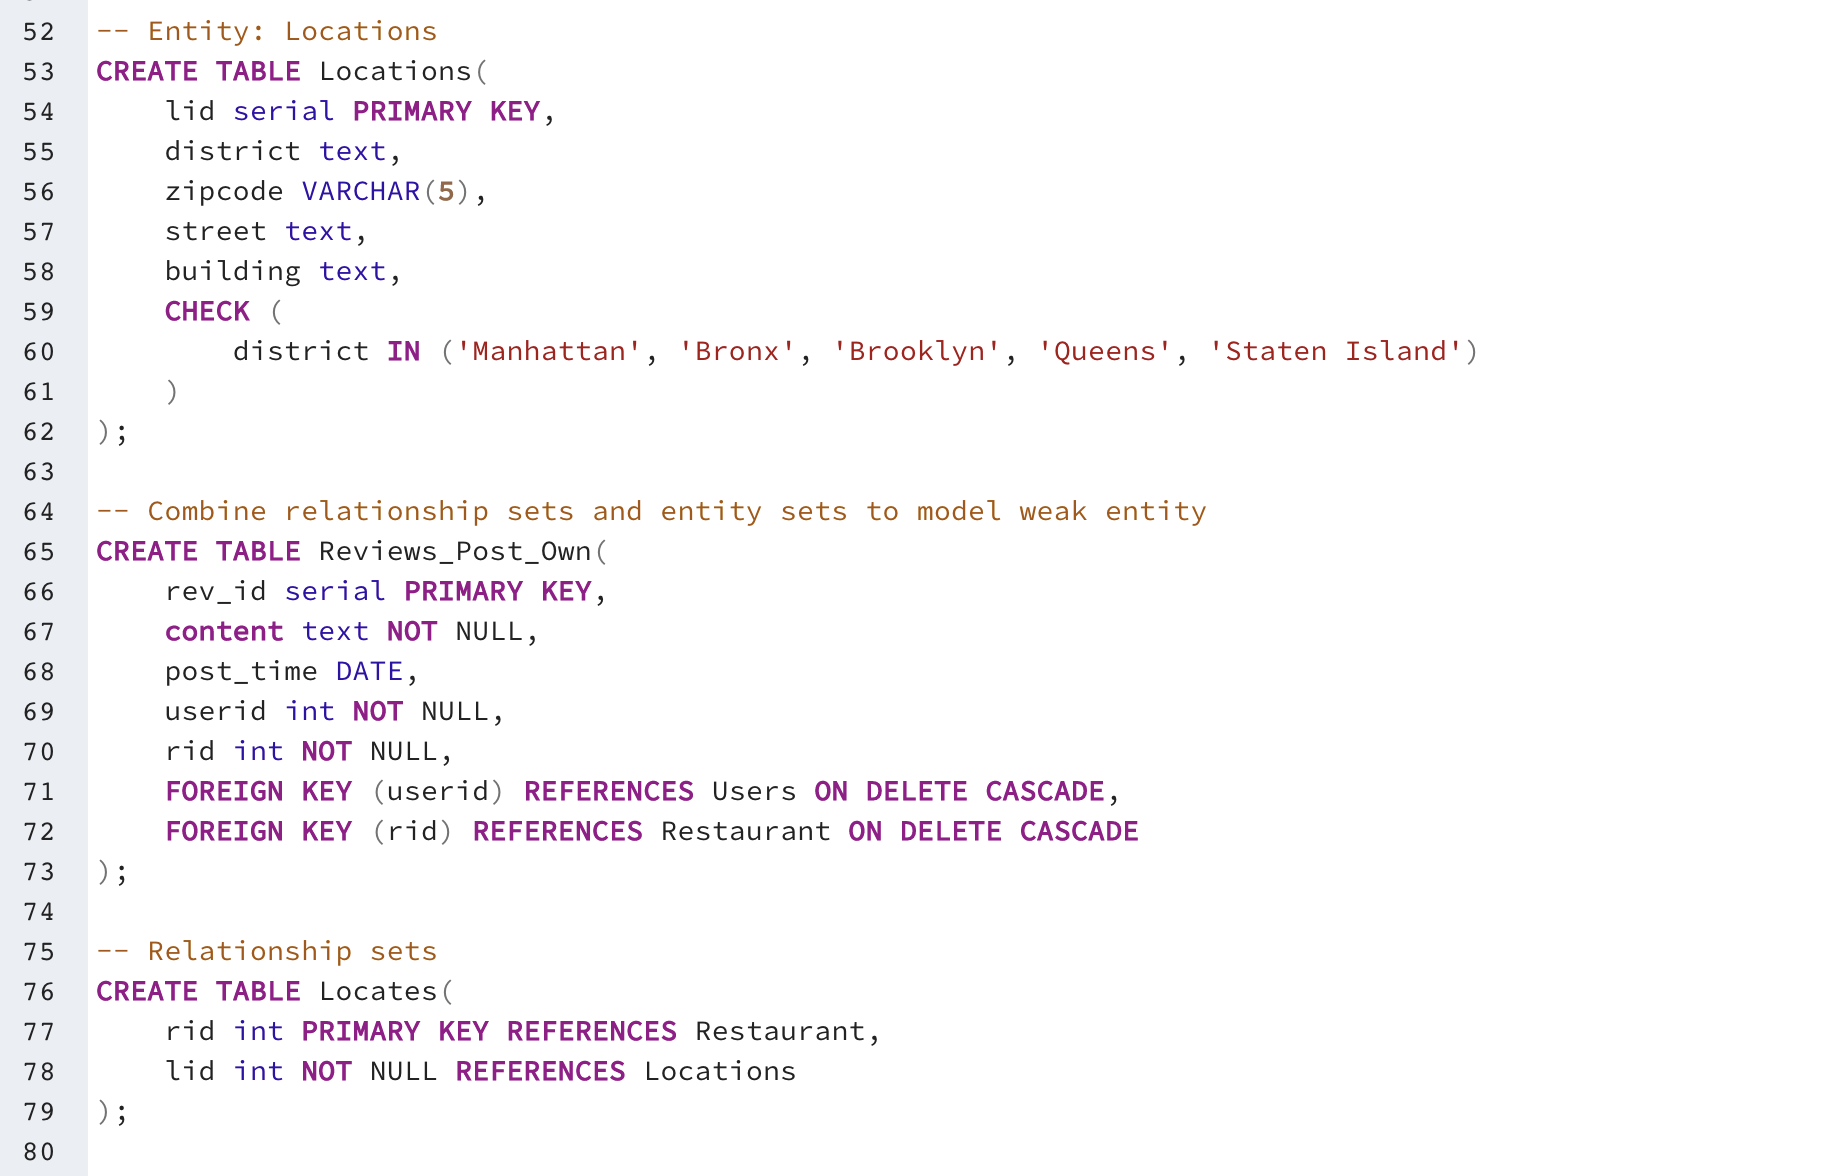
\includegraphics[scale = 0.60]{3.png}
    \caption{Relational Model}
    \label{fig:3}
\end{figure}
\begin{figure}[h]
    \centering
    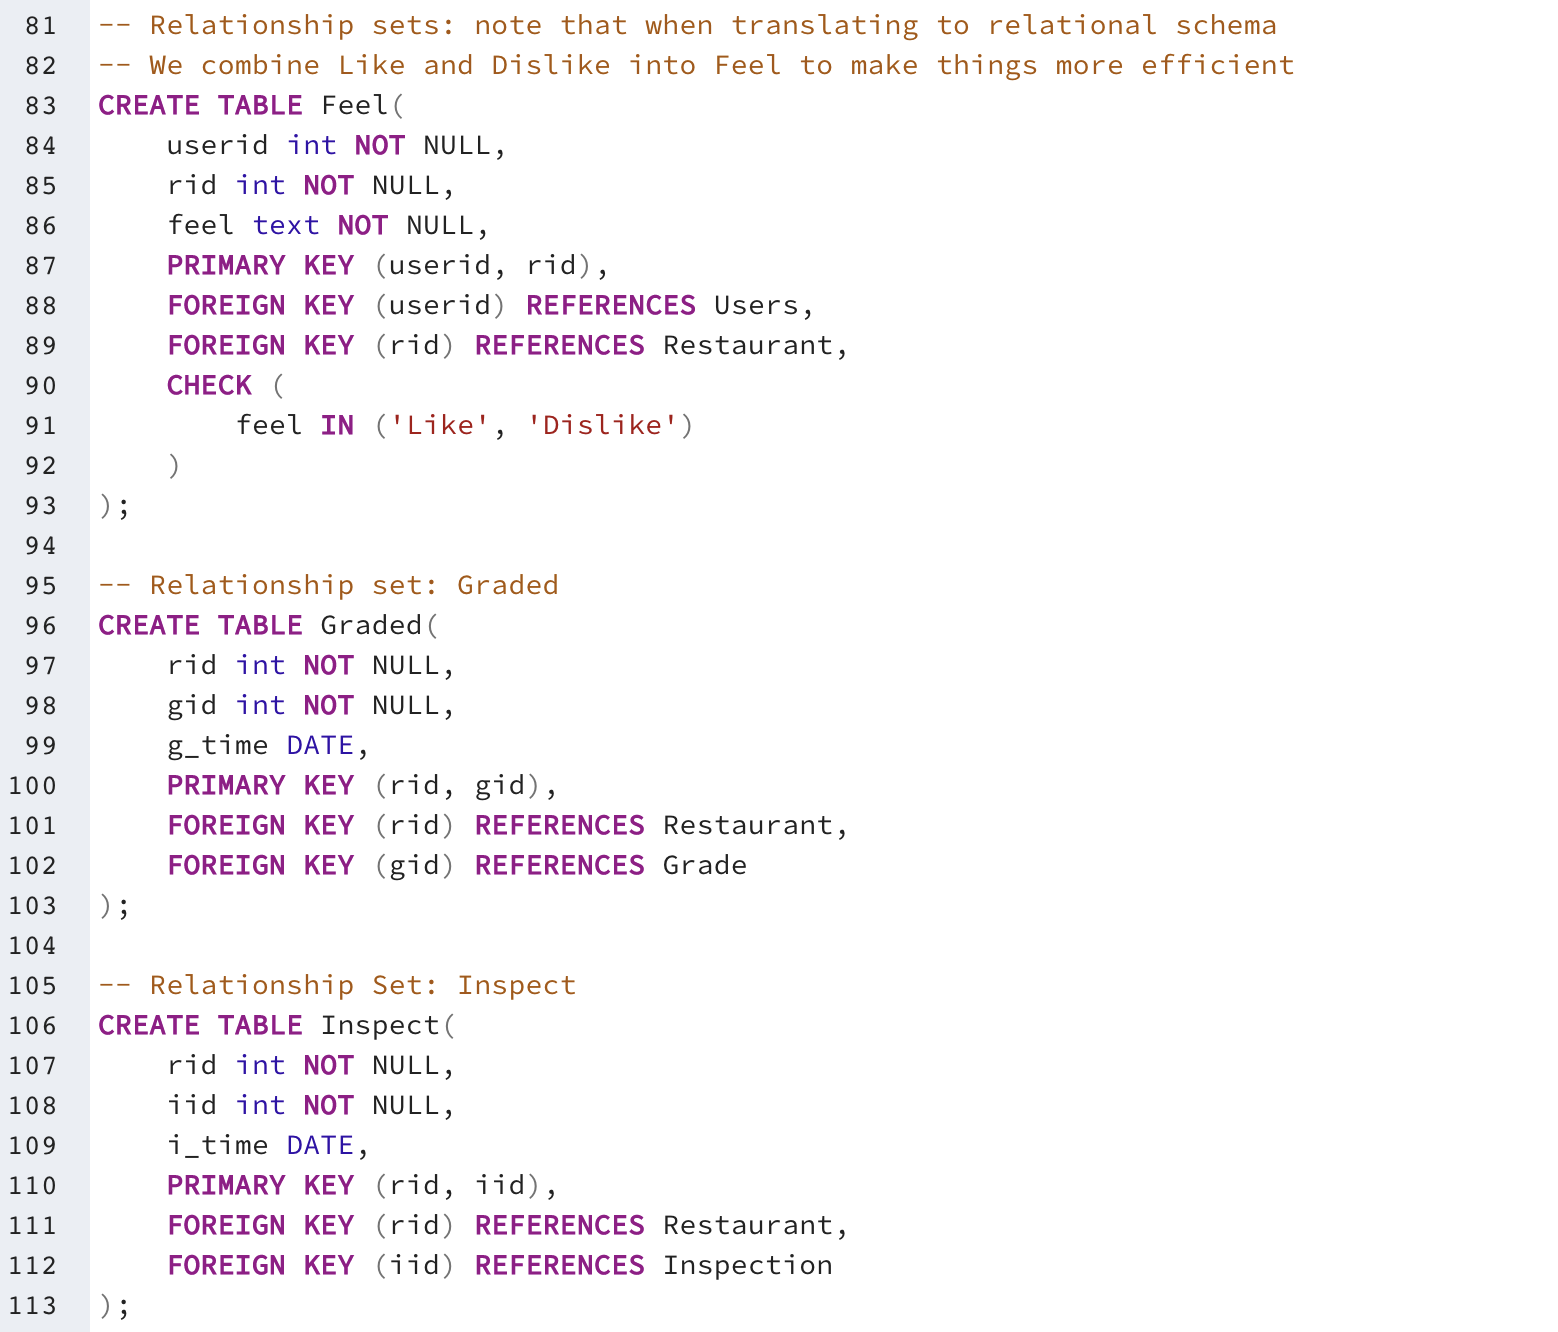
\includegraphics[scale = 0.53]{4.png}
    \caption{Relational Model}
    \label{fig:4}
\end{figure}
\begin{figure}[h]
    \centering
    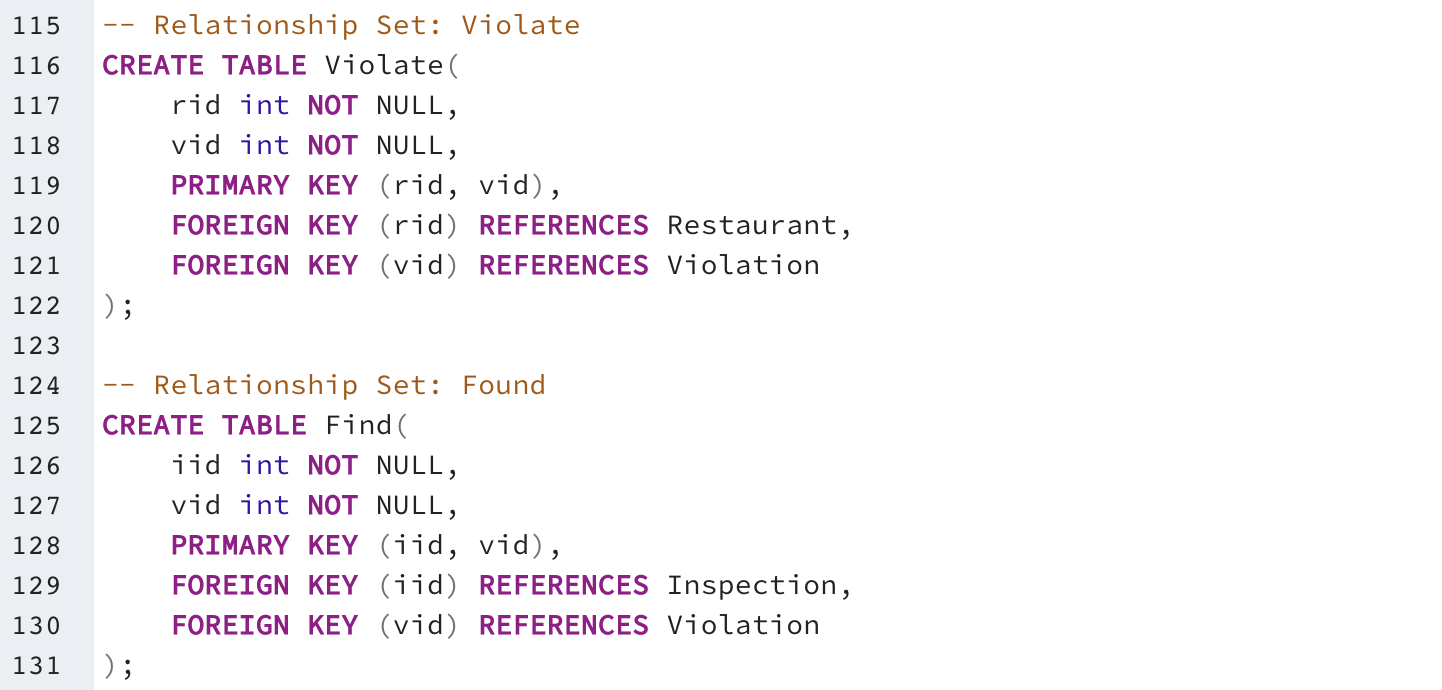
\includegraphics[scale = 0.58]{5.png}
    \caption{Relational Model}
    \label{fig:5}
\end{figure}



\newpage
\section{Appendix A.}
We made the following changes to our ER-Diagram after TA meetings:
\begin{enumerate}
    \item Reconsider the functionality of our application: we change our designs such that our application is not only useful for normal customers but also for government staffs.
    \item As for the ER-Diagram, we remove previous aggregation of the relationship sets \textbf{Inspect} between \textit{Restaurant} and \textit{Inspection} and remodel them with binary relationship sets. Removing unnecessary aggregation simplifies the structure and make things much clearer.
    \item We changed the attributes of users to include more information like their locations, so that our web application can support more functionalities.
    \item We made \textit{Review} a weak entity set of two entity sets \textit{Users} and \textit{Restaurant}. This makes more sense than our previous design where we only made \textit{Review} a weak entity of \textit{Restaurant}.
    \item There are also other changes but are not as significant as the previous four.
\end{enumerate}
\end{document}
